\section{PDCA o Ciclo di Deming}
\label{A}
Ogni processo deve essere organizzato basandosi sul principio del miglioramento continuo (o ciclo di Deming\pedice):

~\newline\textbf{Plan (Pianificare):} viene definito un piano che basandosi sulla definizione di problemi e obiettivi pianifica compiti, assegna responsabilità, studia il caso, analizza le cause della criticità e definisce azioni correttive;

~\newline\textbf{Do (Eseguire):} vengono implementate le attività secondo le linee definite durante la fase Plan;

~\newline\textbf{Check (Valutare):} viene verificato l’esito delle azioni di miglioramento rispetto alle attese;

~\newline\textbf{Act (Agire):} vengono applicate le correzioni necessarie per colmare le carenze rilevate e vengono standardizzate le attività correttamente eseguite.

\begin{figure}[!htbp]
	\centering
	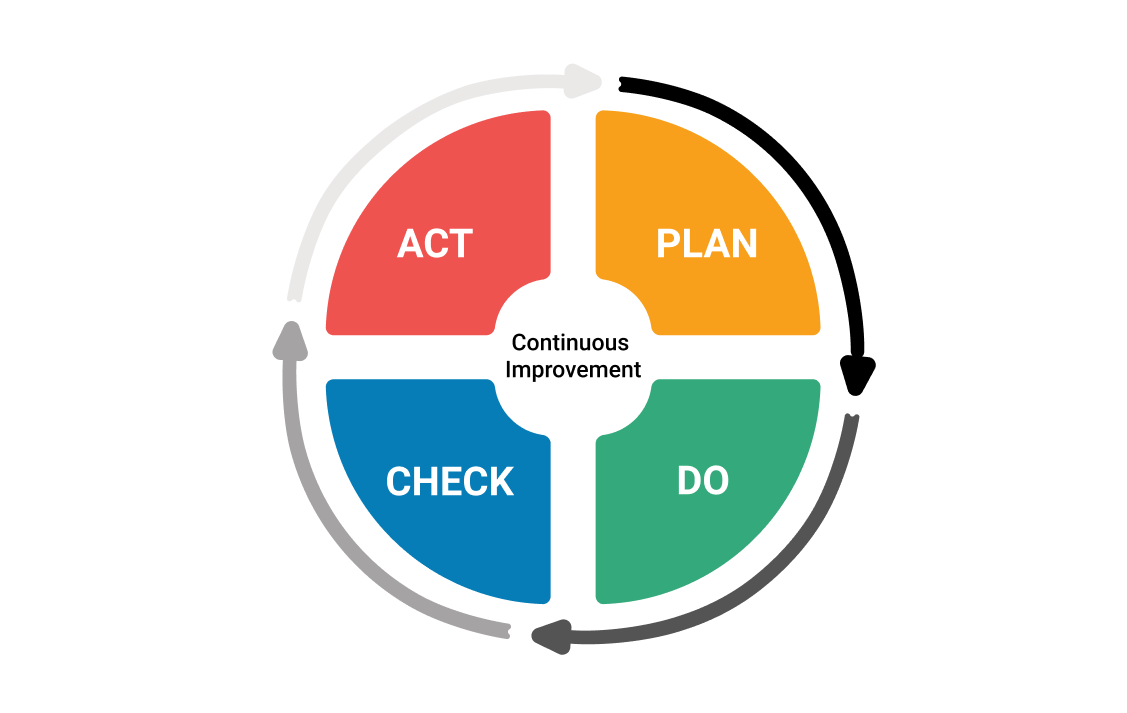
\includegraphics[scale=0.3]{pdca.png}
	\caption{Ciclo di Deming}
\end{figure}

\clearpage

\section{ISO/IEC 15504}
Lo standard ISO/IEC 15504 contiene un modello di riferimento che definisce:
\begin{itemize}
    \item Process dimension;
    \item Capability dimension.
\end{itemize}
La dimensione di processo divide i processi in cinque categorie:
\begin{itemize}
    \item Customer-supplier;
    \item Engineering;
    \item Supporting;
    \item Management;
    \item Organization. 
\end{itemize}
Per ogni processo, lo standard ISO/IEC 15504 definisce dei livelli di capacità:
\begin{itemize}
    \item \textbf{Livello 0:}
    \begin{itemize}
         \item \textbf{Incomplete process:} il processo non è implementato o non raggiunge lo scopo stabilito;
     \end{itemize}
    \item \textbf{Livello 1:}
    \begin{itemize}
         \item \textbf{Performed process:} il processo è implementato e raggiunge lo scopo stabilito;
    \end{itemize}
    \item \textbf{Livello 2:}
    \begin{itemize}
        \item \textbf{Managed process:} il processo è gestito e i prodotti sono stabiliti, controllati e mantenuti;
    \end{itemize}
    \item \textbf{Livello 3:}
    \begin{itemize}
        \item \textbf{Established process:} un processo stabilito si basa su un processo standard;
    \end{itemize}
    \item \textbf{Livello 4:}
    \begin{itemize}
        \item \textbf{Predictable process:} il processo è adottato sistematicamente, entro limiti definiti;
    \end{itemize}
    \item \textbf{Livello 5:}
    \begin{itemize}
        \item \textbf{Optimizing process:} il processo è continuamente migliorato.
    \end{itemize}
\end{itemize}
La capacità dei processi viene misurata attraverso degli attributi di processo:
\begin{itemize}
    \item \textbf{Livello 1:}
        \begin{itemize}
            \item \textbf{Process performance:} capacità di un processo di raggiungere gli obiettivi trasformando input identificabili in output identificabili;
        \end{itemize}
    \item \textbf{Livello 2:}
        \begin{itemize}
            \item \textbf{Performance management:} capacità del processo di elaborare un prodotto coerente con gli obiettivi fissati;
            \item \textbf{Work product management:} capacità del processo di elaborare un prodotto documentato, controllato e verificato;
        \end{itemize}
    \item \textbf{Livello 3:}
        \begin{itemize}
            \item \textbf{Process definition:} l'esecuzione del processo si basa su standard di
            processo per raggiungere i propri obiettivi;
            \item \textbf{Process deployment:} capacità del processo di attingere a risorse tecniche e umane appropriate per essere attuato efficacemente;
        \end{itemize}
    \item \textbf{Livello 4:}
        \begin{itemize}
            \item\textbf{Process measurement:} gli obiettivi e le misure di prodotto e di processo vengono usati per garantire il raggiungimento dei traguardi definiti in supporto ai target aziendali;
           \item \textbf{Process control:} il processo viene controllato tramite misure di prodotto e processo per effettuare correzioni migliorative al processo stesso;
        \end{itemize}
    \item \textbf{Livello 5:}
        \begin{itemize}
            \item \textbf{Process innovation:} i cambiamenti strutturali, di gestione e di esecuzione vengono gestiti in modo controllato per raggiungere i risultati fissati;
            \item \textbf{Process optimization:} le modifiche al processo sono identificate e implementate per garantire il miglioramento continuo nella realizzazione degli obiettivi di business dell'organizzazione.
        \end{itemize}
Ogni attributo consiste di una o più pratiche generiche che sono ulteriormente elaborate in indicatori pratici per aiutare la valutazione delle performance, sotto forma di indici N-P-L-F:
\begin{itemize}
    \item Non soddisfatto (0 - 15\%);
    \item Parzialmente soddisfatto (>15\% - 50\%);
    \item Largamente soddisfatto (>50\% - 85\%);
    \item Totalmente soddisfatto (>85\% - 100\%).
\end{itemize}

\end{itemize}
\clearpage

\section{Metriche}
\label{C}
\subsection{Metriche per la Qualità di processo}
	Verranno  utilizzate  le  seguenti  metriche  per  valutare  l’efficienza  e  l’efficacia  dei processi.
	 	\subsubsection{Schedule Variance (SV)} Indica se si è in linea, in anticipo o in ritardo, rispetto alla schedulazione delle
attività di progetto pianificate nella baseline.
	 	È un indicatore di efficacia soprattutto nei confronti del Cliente.
	 	Se il valore SV ottenuto è positivo significa che il progetto sta procedendo con una
maggiore velocità rispetto a quanto pianificato viceversa se negativo.\newline
	 	\textbf{Misurazione:}
\newline
	 	\[
	 		SV = BCWP-BCWS \newline
	 	\]
 		Dove:
 		\begin{itemize}
 			\item \textbf{BCWP (Budgeted Cost of Work Performed):} È il valore (in giorni
o euro) delle attività realizzate alla data corrente. Rappresenta il valore
prodotto dal progetto ossia la somma di tutte le parti completate e di tutte
le porzioni completate delle parti ancora da terminare;
 			\item \textbf{BCWS (Budgeted Cost of Work Scheduled):} È il costo pianificato (in giorni o euro) per realizzare le attività di progetto alla data corrente. \newline
 		\end{itemize}
	 	\subsubsection{Budget Variance (BV)} Indica se alla data corrente si è speso di più o di meno rispetto a quanto previsto
a budget alla data corrente.
	 	È un indicatore che ha un valore unicamente contabile e finanziario.
	 	Se il valore BV ottenuto è positivo significa che il progetto sta spendendo il proprio
budget con minor velocità di quanto pianificato, viceversa se negativo.\newline
	 	\textbf{Misurazione:}
\newline
	 	\[
	 		BV = BCWS-ACWP \newline
	 	\]
	 	Dove:
	 	\begin{itemize}
	 		\item \textbf{BCWS (Budgeted Cost of Work Scheduled):} È il costo pianificato (in euro) per realizzare le attività di progetto alla data corrente;

	 		\item \textbf{ACWP (Actual Cost of Work Performed):} È il costo effettivamente sostenuto (in euro) alla data corrente.
\newline
	 	\end{itemize}
	 	\textbf{Strategie:} Ogni deficit di SV o BV sarà compensato con la revisione delle attività da svolgere e i requisiti da ottenere, per valutare se nei tempi di calendario stabiliti sia necessario rivedere la programmazione o sia corretta la pianificazione.\\
	 	Il controllo verrà favorito con strumenti come i diagrammi di Gantt in modo tale da avere un cruscotto informativo sull'andamento del progetto e per avere sempre una visone chiara sul lavoro svolto.
	 	\subsubsection{Code Coverage} Verranno usati i seguenti criteri per poter avere una misura di codice testato e verificato:\newline
	 		\begin{itemize}
	 			\item \textbf{Line coverage:} primitiva rispetto alle successive, fornisce un’idea generale del codice. Verificare se ogni linea è stata utilizzata;
	 			\item \textbf{Functional coverage:} Verificare che ogni funzione sia stata chiamata;
	 			\item \textbf{Path coverage:} Verificare che ogni percorso indipendente nel programma sia eseguito almeno una volta;
	 			\item \textbf{Condition coverage:} Verificare che ogni percorso di ogni espressione booleana sia coperto dai test;
	 			\item \textbf{Branch coverage:} Verificare se tutti i possibili branch (derivanti da if e case statement) sono stati eseguiti.
	 		\end{itemize}
	 \textbf{Misurazione:} I test vengono calcolati in percentuale sulla quantità di codice testato e verificato e anche sul totale delle linee di codice scritto, tramite tool automatici descritti in questo documento nelle opportune sezioni.\newline \newline
	 \textbf{Strategie:} Per prevenire bug e vulnerabilità si utilizzano strumenti di code coverage come Jest\footnote{\url{https://jestjs.io/}} per avere una panoramica sullo stato generale del codice prodotto e avere consapevolezza della quantità di codice testato.
	 \subsubsection{Servizi esterni non raggiungibili} Numero totale di giorni in cui siano stati offline o bloccati servizi usati.\newline
		 ~\newline\textbf{Misurazione:} Indice numerico incrementato partendo da zero per ogni giorno
in cui i servizi utilizzati dal gruppo siano risultati totalmente offline per la maggior parte del giorno. I servizi esterni vengono monitorati tramite controllo automatico su \url{statusticker.com}.\newline
		\subsubsection{Rischi non calcolati} Indice numerico che indica la quantità di rischi esterni collegati a quelli presenti nell’attività di
analisi dei rischi rilevati nella corrente fase di progetto.
\newline
		~\newline\textbf{Misurazione:} Indice numerico incrementato partendo da 0 per ogni rischio che
si manifesta senza essere stato individuato precedentemente nella lista di rischi.
		Viene resettato all’inizio di ogni nuova fase di progetto.
		\newline
\subsubsection{Media build Travis per settimana}
Media delle build effettuate settimanalmente sulle diverse repository utilizzate dal gruppo. Potrebbe non coincidere con media dei commit siccome Travis è stato istanziato successivamente all’inizio del progetto.\newline \newline
\textbf{Misurazione:} generato automaticamente tramite bot connesso a Travis.\\
\subsubsection{Build Travis per settimana superate}
Indica la percentuale totale delle build Travis superate per le due repository Github per documentazione e per il prodotto.\newline \newline 
\textbf{Misurazione:} generato automaticamente tramite bot connesso a Travis.\\
\subsubsection{Per tutti i test}
\begin{itemize}
    \item \textbf{Percentuale di test case passati:} indica la percentuale di test case passati,  molto utile per capire a che punto si è nella fase di sviluppo della componente.  La sua formula di misurazione è la seguente:\newline
    \[
		PPT=(\frac{PT}{ET}) \times 100
	\]	
	Dove $PT$ indica il numero di test passati e $ET$ il numero di test eseguiti.
    \item \textbf{Percentuale di test case falliti:} complementare della misu-razione precedente.  La sua formula di misurazione `e la seguente:\newline
    \[
		PFT=(\frac{FT}{ET}) \times 100
	\]	
	Dove $FT$ indica il numero di test falliti e $ET$ il numero di test eseguiti.
    \item \textbf{Tempo medio del team di sviluppo per la risoluzione di errori:} indica  la  quantità  di  tempo  medio  utilizzato  per  risolvere  un  bug dal team di sviluppo,  utile per capire l’impatto medio dell’introduzione di un bug sui tempi di sviluppo.  La sua formula di misurazione è la seguente:\newline
    \[
		TMRE=\frac{TTFB}{TB}
	\]	
	Dove $TTBF$ indica il tempo totale speso per la correzione dei difetti (sviluppo e test) e $TB$ il numero totale di bug trovati.
    \item \textbf{Efficienza  della  progettazione  dei  test:} indica  il  tempo medio per la scrittura di un test, un numero troppo elevato potrebbe indicare che si stanno progettando test troppo complessi o che si sta cercando di  testare  parti  del  codice  superflue.   La  sua  formula  di  misurazione  è  la seguente:\newline
    \[
		TDE=\frac{NTP}{TST}
	\]	
	Dove $NTP$ indica il numero totale di test progettati e $TST$ il tempo per la loro stesura.
    \item \textbf{Contenimento dei difetti:} indica il rapporto percentuale trai bug trovati durante i test e i bug trovati durante l’utilizzo del prodotto.  Un numero  troppo  basso  di  questo  indice  suggerisce  una  scarsa  progettazione dei test, richiedendo un intervento di analisi da parte del team di sviluppo. La sua formula di misurazione è la seguente:\newline
    \[
		CD=(\frac{DTT}{TNDT}) \times 100
	\]	
	Dove $DTT$ indica il numero di difetti trovati durante l’esecuzione dei test, e $TNDT$ la somma dei difetti trovati nei test e quelli trovati durante l’utilizzo del prodotto.

    \item \textbf{Percentuale  di  difetti  sistemati:} indica  la  percentuale  di difetti sistemati sul totale dei difetti rilevati, utile per avere una panoramica dei bug da risolvere:  un numero troppo basso potrebbe costringere il team a fermare lo sviluppo di nuove funzionalità per concentrarsi sulla correzione delle parti già esistenti.  La sua formula di misurazione è la seguente:\newline
    \[
		PDS=(\frac{DS}{DR}) \times 100
	\]	
	Dove $DS$ indica i difetti sistemati mentre $DR$ quelli segnalati.
    \item \textbf{Copertura dei test eseguiti:} indica la percentuale di test già eseguiti sul totale di test da eseguire, utile per monitorare il lavoro del team dei verificatori.  La sua formula di misurazione è la seguente:\newline
    \[
		CTE=(\frac{TE}{TT}) \times 100
	\]	
	Dove $TE$ indica i test eseguiti e $TT$ il numero di test totali.
    \item \textbf{Copertura  dei  requisiti:} indica  la  percentuale  di  requisiti coperti dai test sui requisiti totali, utile per capire quante parti del prodotto finale hanno un test associato, non dà indicazioni sullo stato di avanzamento  del  soddisfacimento  del  requisito.   La  sua  formula  di  misurazione  è la seguente:\newline
    \[
		CR=(\frac{RC}{RT}) \times 100
	\]	
	Dove $RC$ indica il numero di requisiti coperti mentre $RT$ quelli totali.
    \item \textbf{Difetti per requisito:} indica il numero di difetti trovati nel test del requisito, da informazioni sullo stato di soddisfacimento del requisito: se ha 0 difetti, vuol dire che il requisito è stato trovato e considerato senza errori, quindi soddisfatto.  Non essendo calcolabile, la misurazione si mostra come una tabella avente nella prima colonna il nome del requisito,  e nella seconda i difetti ad esso associati.
\end{itemize}

\subsection{Metriche per la Qualità di prodotto}
		Verranno  utilizzate  le  seguenti  metriche  per  valutare  l’efficienza  e  l’efficacia  dei prodotti. \newline Per i documenti sono usate le seguenti metriche:
		\subsubsection{Gulpease Index} 
		\label{C.2.1}
		L’indice Gulpease\pedice è un indice di leggibilità del testo tarato sulla
		lingua italiana. Differentemente da indici di lingua straniera, ha il vantaggio di controllare
la lunghezza delle parole anziché il numero di sillabe per parola, semplificandone il calcolo
automatico.
		Nel complesso, l’indice Gulpease considera la lunghezza delle parole, il numero delle frasi
ed il numero delle parole totali, venendo calcolato con la seguente formula:\newline
		\[
		 	89+\frac{300 \times (numero ~delle ~frasi) - 10 \times (numero ~delle ~lettere)}{(numero ~delle ~parole)}
		\]\newline	
		Il valore risultante è compreso tra 0 e 100, dove un indice più alto corrisponde ad un
indice di leggibilità più semplice.
		Le soglie dei valori dell’indice di leggibilità Gulpease sono:
		\begin{itemize}
			\item inferiore a 80, il documento è difficile da leggere per chi ha la licenza elementare;
			\item  inferiore a 60, il documento è difficile da leggere per chi possiede la licenza media;
			\item inferiore a 40, il documento è difficile da leggere per chi ha un diploma superiore.
			\newline
		\end{itemize}
		\subsubsection{Errori Ortografici} \label{C.2.2} Gli errori ortografici possono essere identificati tramite lo strumento 'Controllo ortografico' presente in TexStudio. Sarà poi compito dei Verificatori correggerli.
\newline
		\subsubsection{Gunning Fog Index} È un indice per misurare la facilità di lettura e di comprensione di un testo. Il numero risultante è un indicatore del numero di anni di educazione formale della quale una persona necessita al fine di leggere il testo con facilità e si misura con la seguente formula:\newline
		\[
		GFI=0.4\times((\frac{numero ~parole}{numero ~frasi})+100\times(\frac{numero ~parole ~complesse}{numero ~parole}))
		\]\newline
		Più l'indice risultante è alto più di difficile comprensione è il testo; in generale un indice minore di 12 si riferisce a un testo destinato a un vasto pubblico.
		\subsubsection{Simple Measure of Gobbledygook (SMOG)}\label{C.2.4} È una misura di leggibilità che stima gli anni di educazione necessari per la comprensione di un testo. Viene calcolato attraverso la seguente formula: \newline
		\[
		SMOG=1.0430\times\sqrt{numero ~di ~polisillabi\times\frac{30}{numero ~di ~frasi}}+3.1291
		\]\newline
		Dove per $polisillabi$ si intendono tutte le parole con tre o più sillabe.
		\newline \newline \newline
		Per il software sono usate le seguenti metriche:\newline
		\subsubsection{Percentuale requisiti fondamentali soddisfatti} Indica la percentuale dei requisiti obbligatori coperti dall’implementazione. La sua
		formula di misurazione è la seguente:\newline
		\[
		PRFS=(\frac{N_{RFS}}{N_{RF}}) \times 100
		\]	
		Dove $N_{RFS}$ è il numero di requisiti fondamentali soddisfatti e $N_{RF}$ è il numero totale
		dei requisiti fondamentali.\clearpage
		\subsubsection{Percentuale requisiti opzionali soddisfatti} Indica la percentuale dei requisiti opzionali coperti dall’implementazione. La sua formula di misurazione è la seguente:\newline
		\[
		PROS=(\frac{N_{ROS}}{N_{RO}}) \times 100
		\]	
		Dove $N_{ROS}$ è il numero di requisiti opzionali soddisfatti e $N_{RO}$ è il numero totale
		dei requisiti opzionali.
		\subsubsection{Mean Time Between Failures (MTBF)} È il valore medio calcolato in unità di tempo tra una failure e la successiva. Viene calcolato attraverso la seguente formula:\newline
		\[
		MTBF=\frac{\sum(inizio ~del ~Downtime - ~inizio ~dell'Uptime)}{numero ~di ~failures}
		\]\newline
		$MTBF$ è un indice molto utile per quantificare l'affidabilità di un sistema.
		\subsubsection{Blocco operazioni non corrette} Indica la percentuale di funzionalità in grado di gestire correttamente i fault che
potrebbero verificarsi. La sua formula di misurazione è la seguente:
\newline
		\[
		BNC=(\frac{N_{FE}}{N_{ON}}) \times 100
		\]	
		Dove $N_{FE}$ è il numero di failure evitati durante i test effettuati e $N_{ON}$ è il numero
di test-case eseguiti che prevedono l’esecuzione di operazioni non corrette, causa
		di possibili failure.
		\subsubsection{Test conclusi in failure} Indica la percentuale di testing che si sono concluse in failure. La sua formula di
misurazione è la seguente:
 \newline
		\[
		TCF=(\frac{N_{FR}}{N_{TE}}) \times 100
		\]	
		Dove $N_{FR}$ è il numero di failure rilevati durante l'attività di testing e $N_{TE}$
è il numero di test-case eseguiti.
		\subsubsection{Tempo di risposta} Indica il tempo medio che intercorre fra la richiesta software di una determinata
funzionalità e la restituzione del risultato all’utente. La sua formula di misurazione
è la seguente:\newline
		\[
		TR=\frac{\sum_{i=1}^{n}T_i}{n}
		\]	
		Dove $T_i$ è il tempo intercorso fra la richiesta \textit{i} di una funzionalità ed il comportamento delle operazioni necessarie a restituire un risultato a tale richiesta.
		\subsubsection{Impatto nuove aggiunte} Indica la percentuale di nuove aggiunte effettuate in risposta a failure che hanno portato
all’introduzione di nuove failure in altre componenti del sistema. La sua formula
		di misurazione è la seguente:
\newline
		\[
		INA=(\frac{N_{FRF}}{N_{FR}}) \times 100
		\]
		Dove $N_{FRF}$ è il numero di failure risolte con l’introduzione di nuove failure e $N_{FR}$
		è il numero di failure risolte.